\documentclass[a4paper,12pt]{article} 
% 使用ctex包支持中文
\usepackage{ctex}
\usepackage{amsmath}
% 开始文档
\usepackage{color}
\usepackage{graphicx}
\begin{document}

% 创建标题页的内容
\title {八省联考导数压轴}
\author{潘世维}
\date{Friday, 20 October 2021}
\maketitle

已知函数 $ f(x)=e^{x}-\sin x-\cos x, g(x)=e^{x}+\sin x+\cos x$


(1) 证明: 当 $ x>-\frac{5 \pi}{4}  $时,$  f(x) \geq 0 $



(2)若 $ g(x) \geq 2+a x $, 求  a 
\begin{flushleft}

(1)\textcolor{red}{证法1:}\\
证明$e^x \ge \sin x + \cos x = \sqrt 2 \sin \left( x + \frac{\pi }{4} \right) $
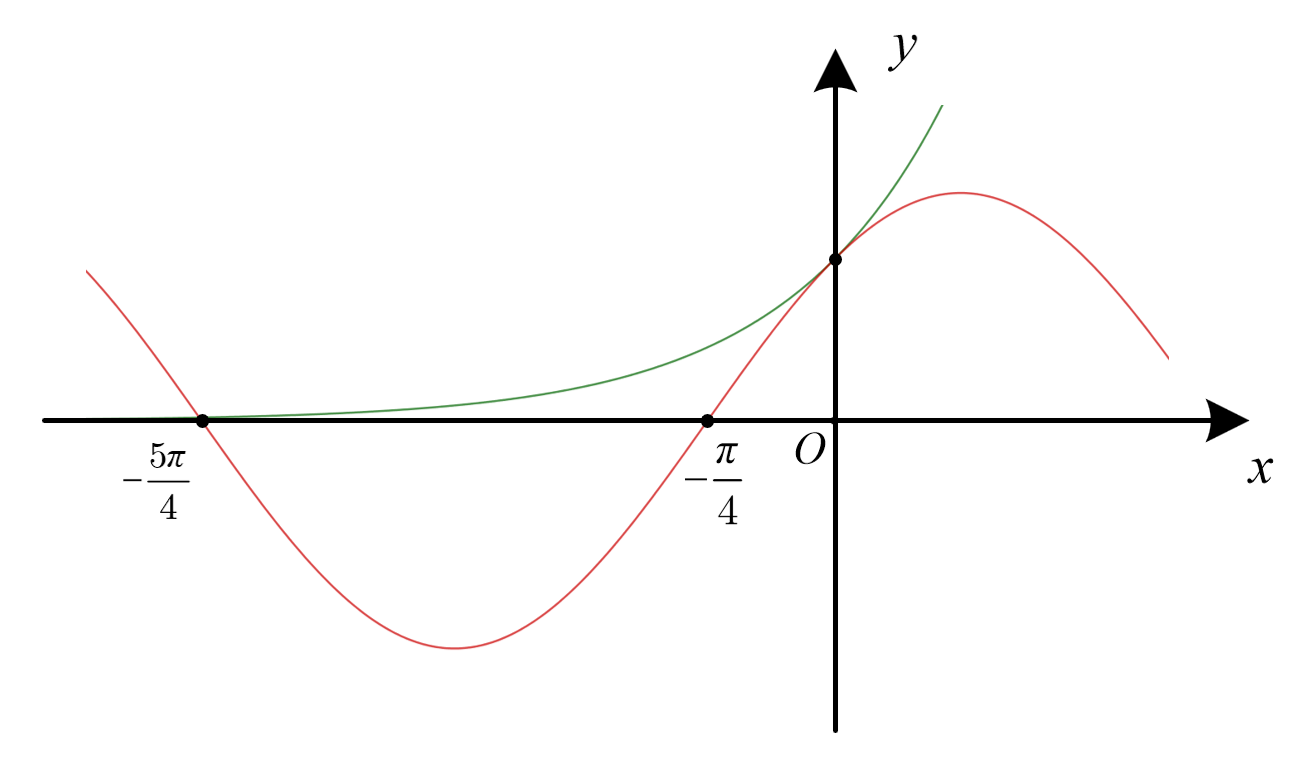
\includegraphics[scale=0.2]{D:/OneDrive/document/8 provinces/pic/pic1.png}\\
①$x \in \left( { - \frac{{5\pi }}{4}, - \frac{\pi }{4}} \right],{e^x} > 0,\sqrt 2 \sin \left( {x + \frac{\pi }{4}} \right) \le 0 \Rightarrow f(x) > 0$

②$x \in \left( { - \frac{\pi }{4},\frac{\pi }{4}} \right),f'(x) = {e^x} - \cos x + \sin x,f''(x) = {e^x} + \sqrt 2 \sin \left( {x + \frac{\pi }{4}} \right) > 0$

$  f'(0) = 0 \Rightarrow f(x) \ge f(0) = 0$

③$\left. {x \in \left[ {\frac{\pi }{4}, + \infty } \right.} \right),{e^x} \ge {e^{\frac{\pi }{4}}},\sin x + \cos x \le \sqrt 2 ,{\left( {{e^{\frac{\pi }{2}}}} \right)^{\frac{1}{2}}} > {2^{\frac{1}{2}}} \Rightarrow f(x) > 0$

\textcolor{red}{证法2:}

证法2:$e^x \ge \sin x + \cos x \Leftrightarrow F(x) = \frac{{\sin x + \cos x}}{{{e^x}}} \le 1 ,F'(x) =  - \frac{{2\sin x}}{{{e^x}}}$

①$x \in \left. {\left( { - \frac{{5\pi }}{4},\pi } \right.} \right],F( - \frac{{5\pi }}{4}) = 0,F(0) = 1,F(x) \le 0$

②$\left. {x \in \left( \pi , + \infty  \right.} \right),f(x) = {e^x} - \sqrt 2 \sin (x + \frac{\pi }{4}) > {e^\pi } - \sqrt 2  > 0$
\\(2)\textcolor{red}{证法1:(同除$e^x$变形):}${e^x} + \sin x + \cos x \ge ax + 2 \Leftrightarrow h(x) = \frac{{ax + 2 - \sin x - \cos x}}{{{e^x}}} \le 1$

$h\left( { - \frac{\pi }{2}} \right) \le 1 \Rightarrow \frac{\pi }{2}a \ge 3 - {e^{ - \frac{\pi }{2}}} > 2 \Rightarrow a > \frac{4}{\pi } >1 $

$h'(x) = \frac{{2\sin x - ax + a - 2}}{{{e^x}}},$记$\varphi (x) = 2\sin x + a(1 - x) - 2,\varphi '(x) = 2\cos x - a$

①$a > 2,\varphi '(x) < 0 \Rightarrow \varphi (x) \downarrow $,又$\varphi (0) = a - 2 > 0,\varphi (\pi ) = (1 - \pi )a - 2 < 0$

$\exists {x_1} \in (0,\pi )$,使$h(x)$在$(0,x_1)\uparrow$,在$(x_1,\pi)\downarrow$,在$x\in(0,x_1)$上有$h(x)>h(0)=1$

②$a = 2,\varphi '(x) = 2\cos x - 2 \le 0,\varphi (x) \downarrow ,\varphi (0) = 0$ ,$h(x)$在$(-\infty,0)\uparrow$,在$(0,+\infty)\downarrow$

$h(x)\ge h(0)=1$

③$a \in (1,2),\varphi '(x)$在$\left( { - \frac{\pi }{2},0} \right) \uparrow ,\varphi '\left( { - \frac{\pi }{2}} \right) =  - a < 0,\varphi '\left( 0 \right) = 2 - a > 0$

$\exists {x_2} \in \left( { - \frac{\pi }{2},0} \right)$,使$\varphi(x)$在$\left( { - \frac{\pi }{2},x_2} \right)\downarrow$,在$(x_2,0)\uparrow$,在$x\in(x_2,0)$上

有$\varphi(x)<\varphi(0)=a-2<0\Rightarrow h(x)$在$(x_2,0)>h(0)=1$

\textcolor{red}{证法2(放缩):}
由(1),当$x>-\frac{5 \pi}{4} $时,有$e^x \ge \sin x + \cos x $

${e^x} \ge 2 + ax - {e^x} \Rightarrow {e^x} \ge \frac{a}{2}a + 1 \Rightarrow a = 2$

下面证明必要性$a = 2,\varphi '(x) = 2\cos x - 2 \le 0,\varphi (x) \downarrow ,\varphi (0) = 0$ ,$h(x)$在$(-\infty,0)\uparrow$,在$(0,+\infty)\downarrow$$h(x)\ge h(0)=1$

\textcolor{red}{证法3(必要性探路):}

$g(x) \ge 0 \Leftrightarrow F(x) = {e^x} + \sin x + \cos x - ax - 2 \ge 0 $ 

$  F(0) = 0 \Rightarrow F'(0) = {e^0} + \cos 0 - \sin 0 - a = 0,a = 2$

下面证明必要性$a = 2,\varphi '(x) = 2\cos x - 2 \le 0,\varphi (x) \downarrow ,\varphi (0) = 0$ ,$h(x)$在$(-\infty,0)\uparrow$,在$(0,+\infty)\downarrow$

$h(x)\ge h(0)=1$
\end{flushleft}
\end{document}  